\documentclass{article}
\usepackage[ruled, linesnumbered]{algorithm2e}
\def\showtopic{Parallel Computing}
\def\showtitle{Communication Avoiding Algorithms\\ in Dense Linear Algebra}
\def\showabs{Comm Avoiding Algs}
\def\showauthor{Ting Lin, 1700010644}
\def\showchead{LIN}
\usepackage{amsmath, amsfonts, amsthm}

\usepackage{graphicx, epstopdf}
\usepackage{color}
\usepackage{geometry, graphicx}
\usepackage{algorithm, algorithmic}
\usepackage{bm}
\usepackage{multirow}
\usepackage{ulem}
\geometry{left = 5em, right = 5em}
\usepackage{listings}
\usepackage{xcolor}
%% notation macro
\newcommand{\F}{\mathcal F}
\newcommand{\T}{\mathcal T}
\newcommand{\I}{\mathcal I}
\newcommand{\U}{\mathcal U}
\newcommand{\R}{\mathbb R}
\renewcommand{\P}{\mathcal P}
\newcommand{\uP}{ \mathcal \uline P}
\newcommand{\B}{\mathcal B}
%\newcommand{\R}{\mathbb R^2}
\newcommand{\Z}{\mathbb Z}
\newcommand{\C}{\mathbb C}
\newcommand{\laplacian}{\triangle}
\newcommand{\grad}{\nabla}
\renewcommand{\div}{\textrm{div~}}

\newcommand{\diff}[2]{\frac{\partial #1}{\partial #2}}
\newcommand{\difff}[3]{\frac{\parial #1^2}{\partial #2 \partial #3}}
\newcommand{\diFF}[2]{\frac{\partial #1^2}{\partial^2 #2}}
\newcommand{\diam}{\text{ diam }}
%% non-noation macro
\newcommand{\IN}{\text{  in  }}
\newcommand{\ON}{\text{  on  }}
\newcommand{\st}{\text{s.t.  }}
\newcommand{\todo}[1]{{\color{red}[TODO:#1]}}
\renewcommand{\Return}{\textbf{return~}}
\newcommand{\Break}{\textbf{break~}}
\newcommand{\Continue}{\textbf{continue~}}
\renewcommand{\And}{\textbf{~and~}}
\newcommand{\Or}{\textbf{~or~}}
%% enviorment
\newtheorem{proposition}{Proposition}
\newtheorem{definition}{Definition}
\newtheorem{corollary}{Corollary}
\newtheorem{remark}{Remark}

\DeclareMathOperator{\argmin}{arg~min}

\renewcommand{\algorithmicrequire}{ \textbf{Input:}} %Use Input in the format of Algorithm
\renewcommand{\algorithmicensure}{ \textbf{Output:}} %UseOutput in the format of Algorithm
\title{\textbf{\showtitle}}
\author{\showauthor}
\usepackage{indentfirst}
\usepackage{fancyhdr}  
\pagestyle{fancy}
\lhead{\textbf {\showtopic} }
\chead{\showchead} 
\rhead{\textbf {\showabs} }
\lfoot{} 
\cfoot{\thepage}
\rfoot{} 
\renewcommand{\headrulewidth}{0.4pt} 
\DeclareMathOperator{\size}{size}
\DeclareMathOperator{\maxd}{\max\nolimits^\delta}
\DeclareMathOperator{\nhi}{\mathcal N_h^{I}}
\DeclareMathOperator{\nhp}{\mathcal N_h^{\partial}}
\DeclareMathOperator{\mind}{\min\nolimits^\delta}
\DeclareMathOperator{\MA}{MA}
\DeclareMathOperator{\MAJ}{MAJ}
\newcommand{\bV}{\mathbb V}
\begin{document}
	\maketitle
	\thispagestyle{fancy}
	\tableofcontents
	
	\section*{}
 In this report we introduce communication avoiding algorithms, which is emerging but powerful computational methods designed for fast computation and expansive communication machine. We focus on dense linear algebra, specifically LU and QR factorization. We show the algorithms, model analysis, and experiment performance. Also, some background information, discussions and possible future works are displayed.
 
 
 \section{Introduction}
 Algorithms often have two parts of costs: Computation and Communication. Communication can happen in move data between either different levels of memory (in sequential case) or processors through network (in parallel case). The (time) cost in communication can be modeled by \textbf{alpha-beta} model, which means that we move $n$ words in one message will take $\alpha + \beta n$ time unit, where $\alpha$ is latency and $\beta$ is the inverse of bandwidth. Moreover, we use $\gamma$ to denote cost time per FLOP. Typically, we have $$\gamma << \beta << \alpha,$$ and the gap grows exponentially, inspired by Moore's law. A good algorithm, even in sequential case, should minimize the communication cost.
 
 
In past two decades, communication avoiding algorithms, including \cite{demmel_communication-optimal_2012,grigori_introduction_nodate,ballard_communication_2014}, have been proposed and well studied. Most of them are superior in theory and practice. In this report, we introduce communication avoiding algorithm in dense linear algebra. We will give several reasons why we focus on dense linear algebra:
\begin{enumerate}
	\item Contrast with Krylov subspace method, dense linear algebra, including LU factorization and QR factorization are easy to analyze its time/energy cost and stability.
	\item Unlike CA algorithms in Sparse linear algebra, algorithms in dense algebra always attains its theoretical lower bound, meaning that we achieve an optimal framework in theory. 
	\item In data science, a faster solver in LU factorization and QR factorization is urgently wanted. Especially for some random methods like random SVD, a lot of techniques for tall and skinny matrices need to be further developed. 
\end{enumerate}

Hence we first focus on dense linear algebra to get some feelings in communication avoiding algorithms. This does not mean that CA methods in sparse linear algebra can be ignored since it is crucial in scientific computing. Existing CA improvement in sparse linear algebra including 
\begin{itemize}
	\item Minimize communication in SpMV (Sparse Matrix-Vector Multiplication). See \cite{demmel_avoiding_2008,mohiyuddin_minimizing_2009}.
	\item Rearrange the computation step in traditional KSM. For example, we postpone the orthogonalization step until the whole Krylov matrix is obtained. Hence a TSQR algorithm can reduce the communication cost. See \cite{hoemmen_communication-avoiding_nodate} for further details.
	\item Change the subspace used in projection methods, for example Enlarged KSM. See \cite{grigori_enlarged_2016}
\end{itemize}

What's more, communication avoiding algorithms arises in several domains, e.g., eigenvalue solver (\cite{Ballard:EECS-2011-14}), preconditioner design (\cite{grigori_communication_2015}), optimization (\cite{soori_avoiding_2017}) and machine learning (\cite{you_ca-svm_2015, Koanantakool:EECS-2017-221}). We will see that in most domain communication avoiding algorithms are far too unexplored and deserve further study.

 \section{Tall Skinny QR and Communication Avoiding QR Factorization}
 We first introduce QR factorization, introduced by \cite{demmel_communication-optimal_2012}. We begin with TSQR, which performs with many more rows than columns. Based on TSQR, we introduce CAQR for general matrices (here we assume that processors grid dimension is $P_r \times P_c$). We will show in table that the latency and communication cost is lower than existing algorithms in LAPACK and ScaLAPACK, with th same numerical stability.
\subsection{TSQR}
The basic idea of parallel TSQR is reduction QR on a binary tree. Suppose we decompose $m\times n$ matrix $A$ into $m/4 \times n$ block rows:
$$A = \begin{bmatrix}
A_0\\A_1\\A_2\\A_3
\end{bmatrix}.$$
We first compute QR decomposition for each block \begin{equation}\left(\begin{array}{c}
A_{0} \\
A_{1} \\
A_{2} \\
A_{3}
\end{array}\right)=\left(\begin{array}{l}
Q_{00} R_{00} \\
Q_{10} R_{10} \\
Q_{20} R_{20} \\
Q_{30} R_{30}
\end{array}\right)\end{equation}

We group them into two pairs, $R_{00}, R_{10}$ and $R_{20}, R_{30}$, and compute the QR decomposition respectively.
\begin{equation}\left(\begin{array}{c}
R_{00} \\
R_{10} \\
\hline R_{20} \\
R_{30}
\end{array}\right)=\left(\begin{array}{c}
R_{00}^* \\
R_{20}^*
\end{array}\right)=\left(\begin{array}{c}
Q_{01} R_{01} \\
\hline R_{11} R_{11}
\end{array}\right)\end{equation}
where $$R_{00}^* = \left(\begin{array}{c}
R_{00} \\
R_{10} \end{array} \right), R_{20}^* =  \left(\begin{array}{c}
R_{20} \\
R_{30} \end{array} \right).$$

For general size, TSQR can be defined recursively along the binary tree. As shown in Matrix Computation, TSQR is as stable as Householder QR, while other QR methods (e.g., Variants of Gram--Schmidt orthogonalization, CholeskyQR) are not so stable.

\subsection{More efficient QR factorization for structured matrices}
In the parallel case, all local QR factorization but the zeroth layer have a particular structure:  they are ($q$, typical 2) vertical stacks of $n\times n$ upper triangular matrices ($x$ denotes some non-zero elements): \begin{equation}\left(\begin{array}{c}
R_{0} \\
R_{1}
\end{array}\right)=\left(\begin{array}{lllll}
x & x & x & x & x \\
& x & x & x & x \\
& & x & x & x \\
& & & x & x \\
& & & & x \\
x & x & x & x & x \\
& x & x & x & x \\
& & x & x & x \\
& & & x & x \\
& & & & x
\end{array}\right)\end{equation}
Since the upper $n\times n$ sub-block is already upper triangular, we propose the following householder QR for these structured matrices.
\begin{algorithm}[htbp]
	\caption{Structured Householder QR}
	\begin{algorithmic}[1]
		\FOR{$j=1$ to $n$}
		\STATE Let $\mathcal I_j$ be the index set $\{j, n+1:n+j, \cdots, (q-1)n+1:(q-1)n+j\}.$
		\STATE $w:=A(\mathcal I_j,j)$
		\STATE $[\tau_j, v] := Householder(w)$ such that $v(1) = 1$
		\STATE $X:= A(\mathcal I_j, j+1:n)$
		\STATE $X := (I - \tau_j vv^T)X$
		\STATE $A(\mathcal I_j \setminus \{j\}, j):= v(2:end)$
		\STATE $A(\mathcal I_j, j+1:n) = X$
		\ENDFOR 
	\end{algorithmic}
\end{algorithm}

We can find that the total cost is about $\frac 23 (q-1)n^3$ flops, about $1/3$ of the original unstructured Householder QR.

Traditional Householder QR is dominated by BLAS 2 operations, which leads to low efficiency in  general. YT representations proposed by Schreiber and van Loan in \cite{wy1989} uses BLAS 3 operation to store the householder reflection:

\begin{algorithm}[htbp]
	\caption{YT representation}
	\label{alg:yt}
	\begin{algorithmic}[1]
		\REQUIRE $n$ Householder reflectors $\rho_j = I - \tau_j v_j v_j^T$
		\FOR{$j=1$ to $n$}
		\IF{$j==1$}
		\STATE $Y:=[v_1]$
		\STATE $T:=[-\tau_1]$
		\ELSE
		\STATE $z := -\tau_j(T(Y^Tv_j))$
		\STATE $Y := [Y v_j]$
		\STATE $T := \begin{bmatrix}
		T & z\\0 & -\tau_j
		\end{bmatrix}$
		\ENDIF
		\ENDFOR
	\end{algorithmic}
\end{algorithm}

$Y$ has no additional computation and storage cost, and $T$ needs about $\frac{2}{3}n^3$ additional flops and $n(n-1)/2$ additional storage per processor. An interesting attribute is that from the above algorithm we can see that we can postpone the computation of $T$ until necessary, only send $Y$ and $\tau$ will reduce the communication cost.
\subsection{CAQR based on TSQR and BLAS 3 Householder}

CAQR is a recursive methods based on TSQR and BLAS 3 Householder transform. Suppose we want to factorize $P_r \times P_c$ block matrix $C$, with each block's data (assumed is a $b\times b$ matrix) is stored in one processor. Intuitively speaking, we first perform TSQR in leftmost column, and then update the local $C$ matrices for the rest processors. We call this step \textbf{trailing matrix update} and describe it before the whole CAQR algorithm.

Our goal is to perform the operation:
\begin{equation}\left(\begin{array}{cc}
R_{0} & C_{0}^{\prime} \\
R_{1} & C_{1}^{\prime}
\end{array}\right)=\left(\begin{array}{cc}
Q R & C_{0}^{\prime} \\
& C_{1}^{\prime}
\end{array}\right)=Q \cdot\left(\begin{array}{cc}
R & \hat{C}_{0}^{\prime} \\
& \hat{C}_{1}^{\prime}
\end{array}\right)\end{equation}
in which $Q$ is the local $Q$ factor and $R$ is the local $R$ factor of $[R_0;R_1]$, and $C_0', C_1'$ is the local matrices (called trailing matrix hereafter) before updating, and $\hat C_0', \hat C_1'$ are those after updating. By YT representation we have 

\begin{equation}\left(\begin{array}{l}
\hat{C}_{0}^{\prime} \\
\hat{C}_{1}^{\prime}
\end{array}\right):=\left(I-\left(\begin{array}{c}
I \\
Y_{1}
\end{array}\right) \cdot {T^{T}} \cdot\left(\begin{array}{c}
I \\
Y_{1}
\end{array}\right)^{T}\right)\left(\begin{array}{c}
C_{0}^{\prime} \\
C_{1}^{\prime}
\end{array}\right)\end{equation}
Here, we suppose that $Y_1$ is on processor $P_1$, $C_0'$ is on processor $P_2$, and $C_1' $ is on processor $P_3$. We propose a straightforward but suboptimal schedule. 
\paragraph{$P_1$'s tasks:}
\begin{itemize}
	\item Send $Y_1$ and $\tau$ to $P_3$
\end{itemize}

\paragraph{$P_2$'s tasks:}
\begin{itemize}
	\item Send $C_0'$ to $P_3$
	\item Receive $W$ from $P_3$
	\item Compute $\hat C_0' = C_0' - W$
\end{itemize}

\paragraph{$P_3$'s tasks:}
\begin{itemize}
	\item Receive $Y_1$ and $\tau$ from $P_1$
	\item Compute $T$ from $Y_1$ and $\tau$ by Algorithm~\ref{alg:yt}. 
	\item Compute $W = T^T(C_0' + Y_1^TC_1')$
	\item Send $W$ to $P_2$ 
	\item Compute $\hat C_1' =C_1' - Y_1W$
\end{itemize}
The schedule leads to some load imbalance, since $P_3$ performs much more computation than $P_2$. But this will be alleviated if we overlap the communication and computation in  CAQR algorithm. 

CAQR is defined inductively. We assume that first $j-1$ iterations have been performed. Hence $Y$ part and $R$ part is inactive now. 
\begin{figure}[htbp]
	\centering 
	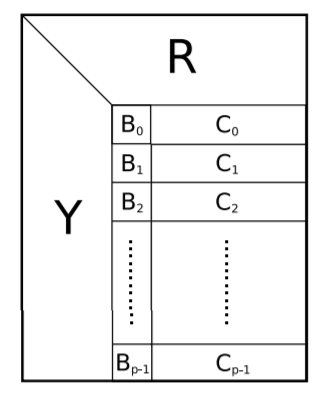
\includegraphics[scale=0.4]{CAQR.png}
\end{figure}
We first use TSQR to factorize the stacked block $B_0, \cdots B_{p-1}$, and then update the trailing matrices in $C_{0}, \cdots, C_{p-1}$. Here we use a butterfly-like techniques to make sure that trailing matrix updating is compatible with TSQR step. We show that in 1 iteration how we update the trailing matrix and obtain the desired factor. Here we suppose we deal with matrix of size $m\times n = P_rb \times P_cb$. For simplicity, we denote the processors in leftmost column are indexed with $0,1,P_r-1$. We use several notations to describe our bufferfly-like strategy.

\begin{itemize}
	\item $level(i,k) = [i/2^k]$ denotes the node at level $k$ of the reduction. The initial stage is $i=0$, i.e., with no communication.
	\item $first\_proc(i,k) = 2^klevel(i,k)$ is the index of first processor in the node that $i$ belongs to.
	\item $target(i,k) = first\_proc(i,k) + (i + 2^{k-1}) \mod 2^k$ is the index of the processor with which $i$ exchange data at level $k$ of the butterfly all-reduction algorithm.
	\item $target\_first\_proc(i,k) = target(first\_proc(i,k))$
\end{itemize}

We first restate TSQR more clearly, see Algorithm~\ref{alg:tsqr}
\begin{algorithm}[htbp]
	\caption{TSQR}
	\label{alg:tsqr}
	\begin{algorithmic}[1]
		\STATE For each processor, compute $A_p = Q_{p,0}R_{p,0}$ locally.
		\FOR{$k = 1: \log P$}
		\IF{$i == target\_first\_proc(i,k) ~~or ~~first\_proc(i,k)$}
		\STATE $\phi = first\_proc(i,k), \tau =  target\_first\_proc(i,k)$
		\ELSE
		\STATE \Continue
		\ENDIF
		\STATE $l = level(i,k)$
		\STATE $\phi$ and $\tau$ exchange their data.
		\STATE Compute the structured Householder QR. $\begin{bmatrix}
		A_{\phi} \\ A_{\tau}
		\end{bmatrix} = Q_{l,k}R_{l,k}$
		\ENDFOR
	\end{algorithmic}
\end{algorithm}

\begin{algorithm}[htbp]
	\caption{one step CAQR}
	\label{alg:caqr}
	\begin{algorithmic}[1]
		\STATE Perform TSQR on $[C_{0}, C_{1}, \cdots C_{P_r-1}]$, storing $Y_{pk}$ and $\tau_{pk}$ in each processor 
		\STATE For each processor in leftmost column, broadcast its $Y_{pk}$ and $\tau_{pk}$ to all processors share the same row with $p$. 
		\STATE Form $T_{p,0}$ locally and update the trailing matrix.
		\FOR{$k=1:\log P_r$}
			\IF{$p==first\_proc(p,k)$ or $target\_first\_proc(p,k)$}
			\STATE Processors in the same row as $target\_first\_proc(p,k)$ form $T_{level(p,k),k}$ locally. Compute $W = Y^T_{level(p,k),k}C_{target\_first\_proc(p,k)}$ locally.
			\STATE Each processor in the same process row as $first\_proc(p,k)$ sends to the processor in the same column and belonging to the row of $target\_first\_proc(p,k)$, the $C_{first\_proc(p,k)}$.
			\STATE Compute \begin{equation}W=T_{\text {level}(p, k), k}^{T}\left(C_{\text {first\_ {proc}}(p, k)}+W\right)\end{equation} locally.
			\STATE Send back $W$ from the row $target\_first\_proc(p,k)$ to $first\_proc(p,k)$ the local $W$.
			\STATE Update the $target\_first\_proc(p,k)$'s trailing matrix: $C_{target\_first\_proc(p,k)} = C_{target\_first\_proc(p,k)} - Y_{level(p,k),k}W$
			\STATE Update the $first\_proc(p,k)$'s trailing matrix: $C_{first\_proc(p,k)} = C_{first\_proc(p,k)} - W$
			
			\ENDIF
		\ENDFOR
	\end{algorithmic}
\end{algorithm}

Notice that in Algorithm~\ref{alg:caqr} line 5 and line 6, line 8 and line 9 can overlap to reduce the cost time.
\subsection{Model Analysis}
In this subsection we analyze the cost of TSQR and CAQR, comparing with PDGEQRF in ScaLAPACK.
\paragraph{TSQR} A parallel TSQR factorization on a binary reduction tree (just what we introduced) performs the following computations along the critical path:
\begin{itemize}
	\item One local QR of fully dense $m/P \times n$ matrix  $ \to (2mn^2/P - 2n^3/3 + O(mn/P)$ FLOPs)
	\item $\log P $ structured Householder QR, each $\to\frac 23 n^3 + O(n^2)$ FLOPs)
\end{itemize}
Thus the total flop count is \begin{equation}\frac{2 m n^{2}}{P}-\frac{2n^{3}}{3}+\frac{2}{3} n^{3} \log P+O\left(\frac{m n}{P}\right).\end{equation}
the total message count is $\log P$, the total words communicated is 
$\log P \frac{n(n+1)}{2}$.

\paragraph{Updating trailing matrix} We model the performance of the parallel CAQR algrithms. We assume no overlapping of computation and communication. We recall our assumption: the matrix $A$ is stored in 2-D block cyclic layout on $P_r \times P_c$ grid of processors, and we assume $P_r$ evenly divides $m$ and $P_c$ evenly divides $n$. Each block is $b \times b$ matrix.

We start counting FLOPs in updating the trailing matrix.
First we consider the cost forming $T$ from $Y$ and $\tau$: from $T(1:j-1,1:j-1)$ to $T(1:j,1:j)$ we need to compute $\tau T(1:j-1,1:j-1)Y_1(1:j-1,1:j-1)^Tv_j(n+1:n+j)$ leading to a cost of $(j-1)(j) + 2\frac{(j-1)^2}{2}$. Summing up $j$ from $1$ to $n$ we obtain the FLOPS of forming $T$ is about $\frac{2}{3}n^3 + l.o.t$.
Next we counts the FLOPs in updating trailing matrix: 

\begin{equation}\left(\begin{array}{l}
\hat{C}_{0}^{\prime} \\
\hat{C}_{1}^{\prime}
\end{array}\right):=\left(I-\left(\begin{array}{c}
I \\
Y_{1}
\end{array}\right) \cdot {T^{T}} \cdot\left(\begin{array}{c}
I \\
Y_{1}
\end{array}\right)^{T}\right)\left(\begin{array}{c}
C_{0}^{\prime} \\
C_{1}^{\prime}
\end{array}\right)\end{equation}
in which $Y_1$ is $n\times n$ upper triangular and $C_0', C_1'$ is $n\times q$. We outline the costs which is $3n^2q+6nq$ in total:

\begin{itemize}
	\item Compute $W = T^T(C_0' + Y_1^TC_1') \to n(n+1)q + nq + n(n+1)q$ FLOPs
	\item Compute $\hat C_0' = C_0' - W \to nq$ FLOPs
	\item Compute $\hat C_1' =C_1' - Y_1W \to n(n+2)q$ FLOPs 
\end{itemize}

\paragraph{CAQR} We are ready for CAQR.  suppose $m_j = (m-1+j)b, n_j = (n-1+j)b$ be the size of active matrix in the $j-th$ iteration 

\begin{enumerate}
	\item TSQR on leftmost column: 
	
	\#FLOPs  $\approx 2b^3+ \frac{2b^3}{3} \log P_r~~~~$    \#messages  $\approx \log P_r~~~~$
		\#words $\approx \frac{b^2}{2} \log P_r$
	
	\item Broadcasting Householder vector and multipliers along rows: 
	
	
		\#FLOPs  $\approx 0~~~~$
		\#messages  $\approx \log P_c~~~~$
	\#words $\approx (\frac{b^2}{2} + b) \log P_r \log P_c$
	\item First update the trailing matrix locally
	
		\#FLOPs  $\approx \frac{11}{3}b^3~~~~$
	\#messages  $\approx 0~~~~$
	\#words $\approx 0$
	\item Butterfly all-reduce at stage $k$,$p==first\_proc(p,k)$ or $target\_first\_proc(p,k)$:
	 \begin{enumerate}
	 	\item  Processors in the same row as $target\_first\_proc(p,k)$ form $T_{level(p,k),k}$ locally. Compute $W = Y^T_{level(p,k),k}C_{target\_first\_proc(p,k)}$ locally. 
	 	
	 			\#FLOPs  $\approx \frac{5}{3}b^3~~~~$
	 	\#messages  $\approx 0~~~~$
	 	\#words $\approx 0$
	 	
	 	\item  Each processor in the same process row as $first\_proc(p,k)$ sends to the processor in the same column and belonging to the row of $target\_first\_proc(p,k)$, the $C_{first\_proc(p,k)}$.
	 	
	 		 			\#FLOPs  $0~~~~$
	 	\#messages  $1~~~~$
	 	\#words $b^2$
	 	\item  Compute \begin{equation}W=T_{\text {level}(p, k), k}^{T}\left(C_{\text {first\_ {proc}}(p, k)}+W\right)\end{equation} locally.
	 	
	 	\#FLOPs  $\approx b^3~~~~$
	 	\#messages  $0~~~~$
	 	\#words $0$
	 	\item  Send back $W$ from the row $target\_first\_proc(p,k)$ to $first\_proc(p,k)$ the local $W$.
	 	
	 		 	\#FLOPs  $0~~~~$
	 	\#messages  $1~~~~$
	 	\#words $b^2$
	 	\item Update the $target\_first\_proc(p,k)$'s trailing matrix: $C_{target\_first\_proc(p,k)} = C_{target\_first\_proc(p,k)} - Y_{level(p,k),k}W$
	 	\item  Update the $first\_proc(p,k)$'s trailing matrix: $C_{first\_proc(p,k)} = C_{first\_proc(p,k)} - W$
	 	
	 	\#FLOPs  $\approx b^3~~~~$
	 	\#messages  $0~~~~$
	 	\#words $0$
	 \end{enumerate}
\end{enumerate}
In total, we have 
	 	\#FLOPs  $\approx 2b^3P_r + 8b^3P_r\log P_r~~~~$
\#messages  $\approx P_r(3\log P_r + \log P_c)~~~~$
\#words $\approx \frac{5b^2}{2} P_r\log P_r + \frac{b^2}{2} P_r \log P_r \log P_c$.
\subsection{Performance test}

We select the experiment results in \cite{demmel_communication-optimal_2012}. Consider a distributed memory, in-DRAM on each node. Two machines are used :
\begin{enumerate}
	\item\textbf{ Pentium III cluster (“Beowulf”)}
	
	Operated by the University of Colorado at Denver and the Health
	Sciences Center
	
	35 dual-socket 900 MHz Pentium III nodes with Dolphin interconnect
	
	Floating-point rate: 900 Mflop/s per processor, peak
	
	Network latency: less than 2.7 $\mu$s, benchmarked
	
	 Network bandwidth: 350 MB/s, benchmarked upper bound
	 \item \textbf{IBM BlueGene/L (``Frost'')}


Operated by the National Center for Atmospheric Research

 One BlueGene/L rack with 1024 700 MHz compute CPUs

 Floating-point rate: 2.8 Gflop/s per processor, peak

 Network5
latency: 1.5 $\mu$s, hardware

 Network one-way bandwidth: 350 MB/s, hardware

\end{enumerate}

\begin{figure}[htbp]
	\centering
	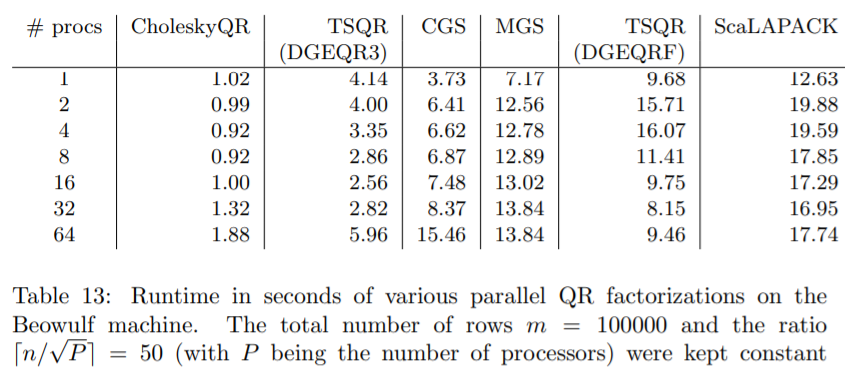
\includegraphics[scale=.6]{TSQR_res1.png}
	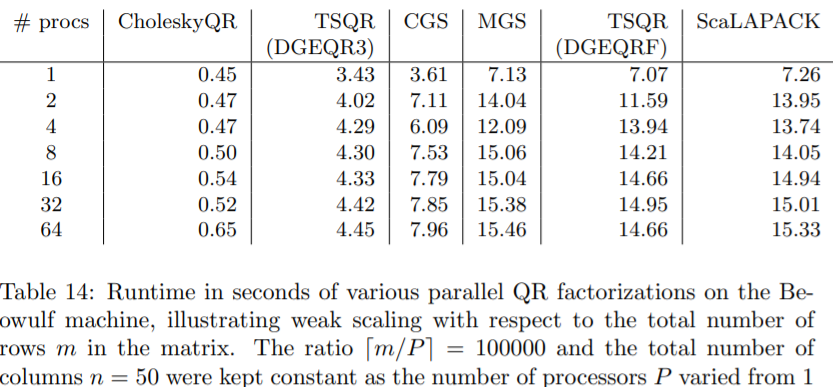
\includegraphics[scale=.6]{TSQR_res2.png}
\end{figure}
Notice that in Table 13 and 14,  Pentium II have relatively slow processors with a relative low-latency interconnect, while TSQR was optimized for the opposite case of fast processors and expensive communication. However, it still outperforms than ScaLAPACK.

For CAQR, we test the best choice of CAQR and PDGEQRF (in ScaLAPACK) in IBM Power 5, Peta and Grid.

\begin{figure}[htbp]
	\centering
	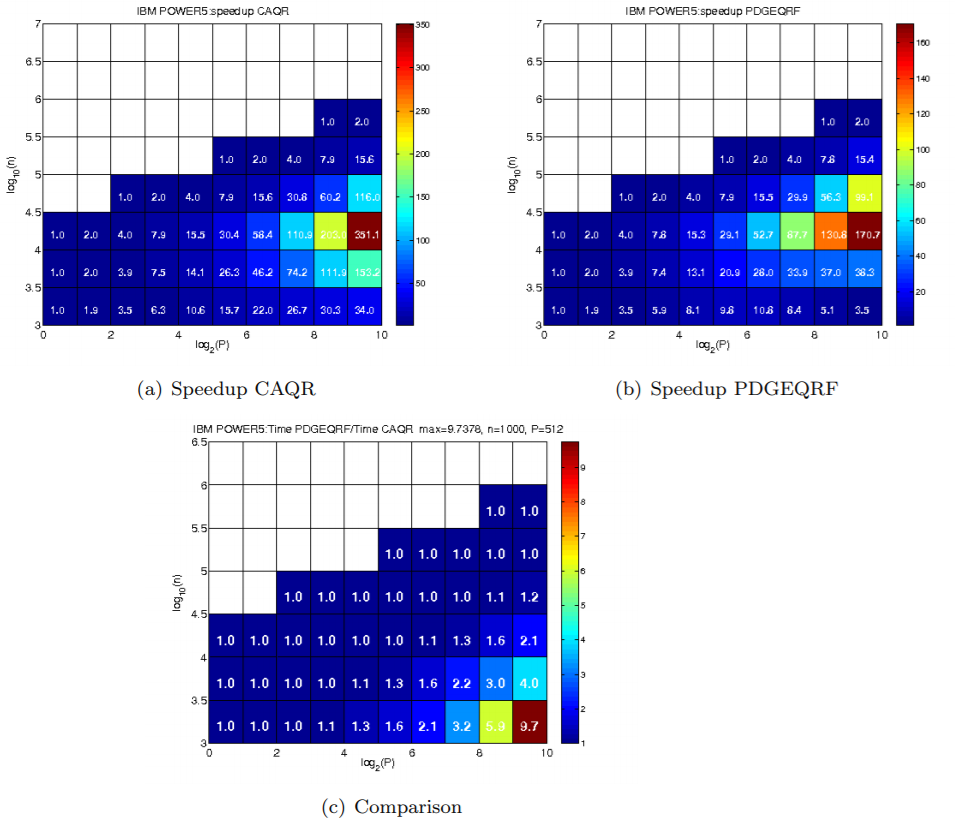
\includegraphics[scale=.6]{CAQR_res1.png}
\end{figure}
\begin{figure}[htbp]
	\centering
	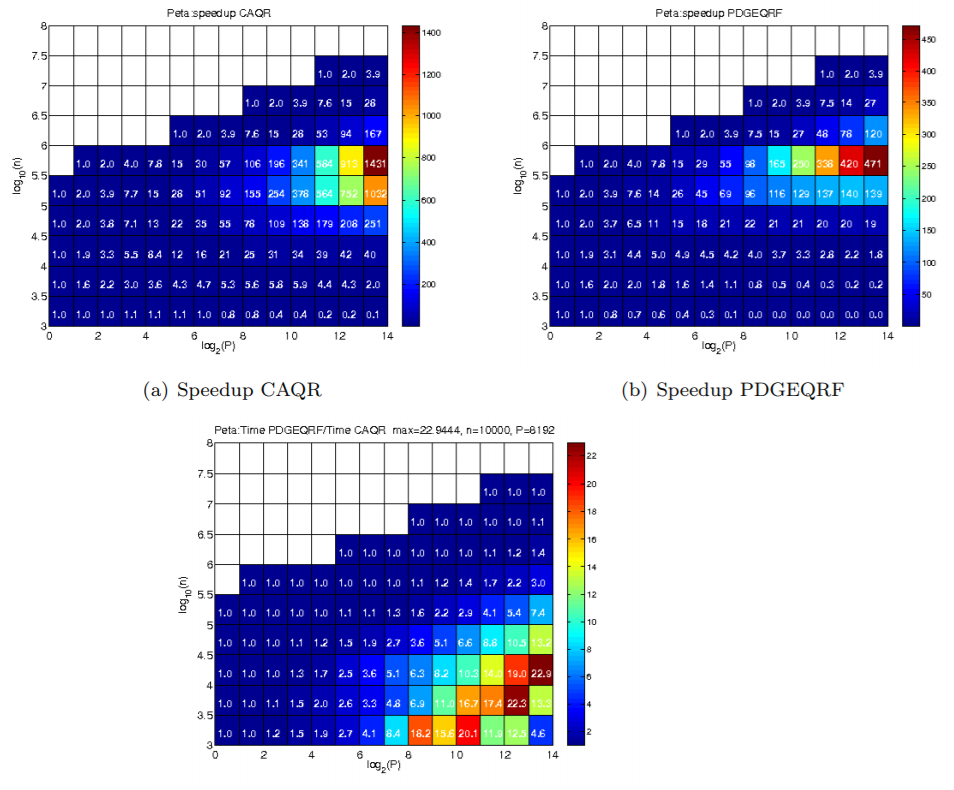
\includegraphics[scale=.6]{CAQR_res2.png}
\end{figure}
\begin{figure}[htbp]
	\centering
	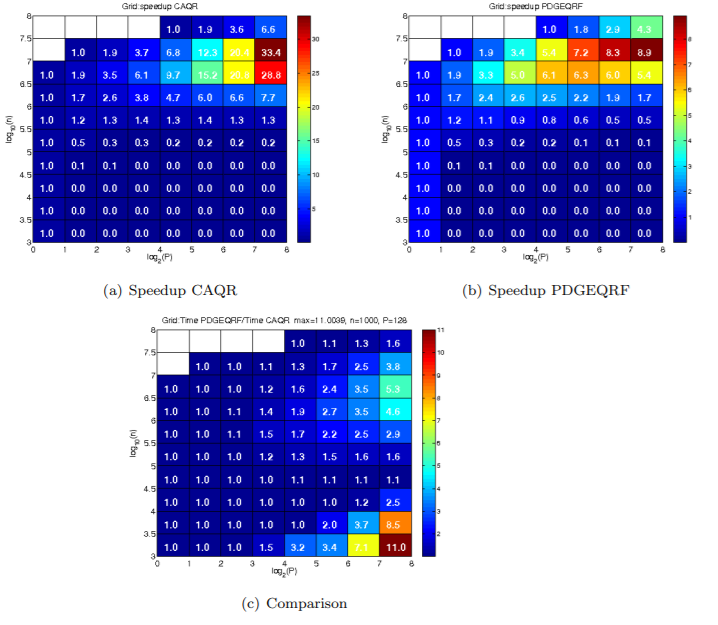
\includegraphics[scale=.7]{CAQR_res3.png}
\end{figure}
 \section{Communication Avoiding LU Factorization}
 CALU is proposed in a rather similar way (\cite{grigori_communication_2008, grigori_calu_2011}): we first introduce Tall and Skinny LU factorization and then consider the update step by a butterfly all-reduced algorithm. The latter, called GEPP, will be more technical than we encountered in QR.

\subsection{TSLU}
We first recall Gaussian Elimination with Partial Pivoting called GEPP. Suppose we have two local $A$ with factorization $\Pi_{0}A_0 = L_0 U_0$ and $\Pi_1A_1 = L_1 U_1$. Then the reduction step we need to compute GEPP about following stacked matrix 
$$A = \begin{bmatrix}
\Pi_0A_0 \\ \Pi_1 A_1
\end{bmatrix}
$$

The algorithmic statement can refer Algorithm~\ref{tslu}.

\begin{algorithm}[htbp]
	\caption{TSLU}
	\label{alg:tslu}
	\begin{algorithmic}[1]
		\STATE For each processor, compute $\Pi_{p,0}A_p = L_{p,0}U_{p,0}$ locally. Let $B_i = (\Pi_{p,0}A_i)(1:b,1:b)$
		\FOR{$k = 1: \log P$}
		\IF{$i \ge target\_first\_proc(i,k)$}
		\STATE $\phi = target(i,k), \tau =  i$
		\ELSE
		\STATE  $\tau = target(i,k), \phi =  i$
		\ENDIF
		\STATE $l = level(i,k)$
		\STATE $\phi$ and $\tau$ exchange their data.
		\STATE Compute the LU decomposition. $\Pi_{l,k}\begin{bmatrix}
		B_{\phi} \\ B_{\tau}
		\end{bmatrix} = L_{l,k}R_{l,k}$
		\STATE Let $B_i = \left(\Pi_{l,k}\begin{bmatrix}
		B_{\phi} \\ B_{\tau}
		\end{bmatrix}\right)(1:b,1:b)$
		\ENDFOR
		\STATE The final permutation is $\Pi = \Pi_{\log P} \cdots \Pi_0$
		\STATE $U = U_{0,\log P}$
		\STATE solve $L = AU^{-1}$ locally.
	\end{algorithmic}
\end{algorithm}
\subsection{Whole CALU and Model Analysis}
At each iteration, we compute TSLU factorization of the leftmost column. Then we broadcast the pivot information and perform LU iteration. 

\begin{algorithm}[htbp]
	\caption{one step CALU}
	\label{alg:calu}
	\begin{algorithmic}[1]
		\STATE Perform TSLU on the leftmost block column.
		\STATE Broadcast the pivot information into all processors. For all processors in leftmost column, broadcast its $L$ along the processor row. 
		\STATE Swap rows according to pivot information.
		\STATE For all processors in uppermost row, update trailing matrix $A = L^{-1}A$. Then broadcast it along processor column, denoted as $U$.
		\STATE For all rest processors, update $A = A - LU$.
	\end{algorithmic}
\end{algorithm}

\subsection{Model Analysis}
We summarize the cost of TSLU and CALU for short, since the counting is similar to those in QR, again we omit all lower order terms.

For TSLU, we need about $2mb^2/P + \frac{2b^3}{3}(\log P)$ FLOPs, $\log P$ messages , and $\frac{b^2}{2} \log P$ words to communicate.

For CALU, we need about $2b^3P_r + \frac{2b^3}{3}P_r(\log P_r) + 4b^2 P_r \log P_r$ FLOPs,$P_r(2\log P_r + 2\log P_c)$ messages, $b^2P_r(\log P_r + \log P_c)$ words to communicate.
\subsection{Performance}
We show the result in \cite{grigori_calu_2011}
and references therein, see Table 3 and 4.

\begin{figure}[htbp]
	\centering
	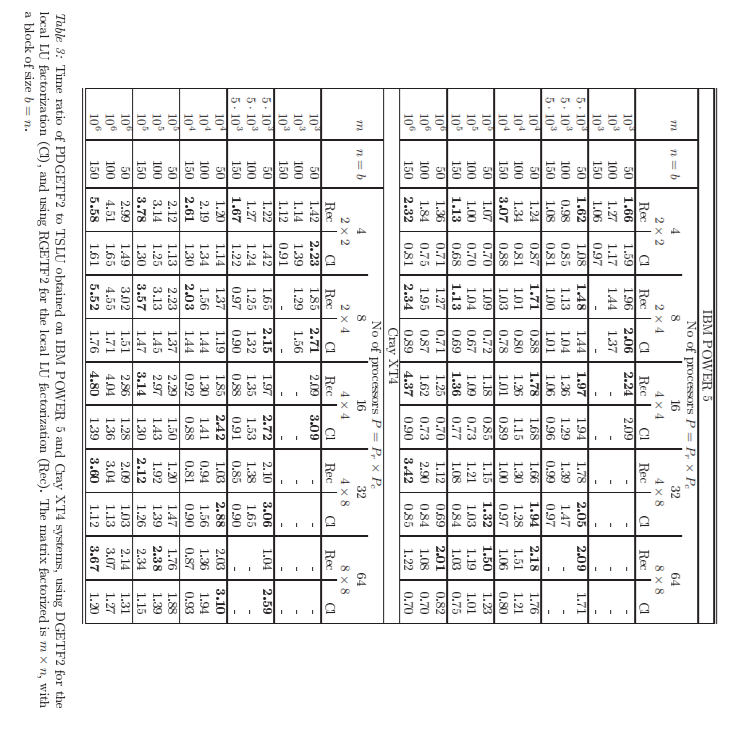
\includegraphics[scale=.6]{TSLU_res.png}
\end{figure}
\begin{figure}[htbp]
	\centering
	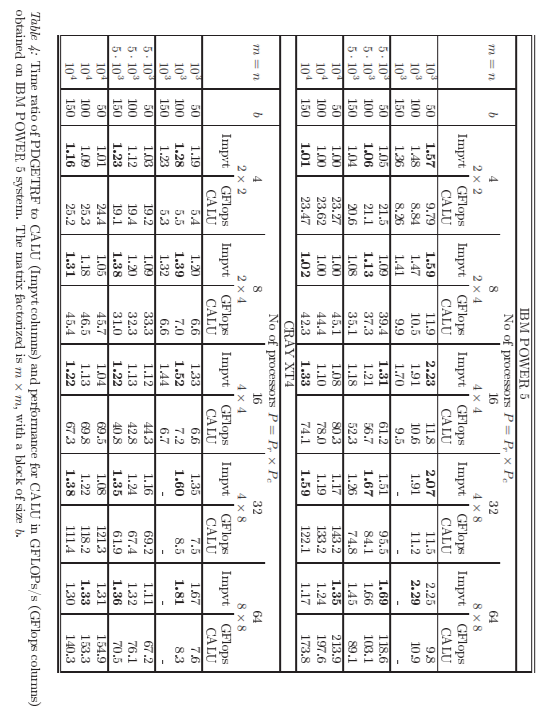
\includegraphics[scale=.6]{CALU_res.png}
\end{figure}


 \section{Discussions and Possible Future Work}
 Communication Avoiding algorithms express great power in both theory and practice. However, even for dense linear algebra (which we attained lower bound already), we still have a lot of research topic: for example implementation of CA algorithm into various multi-/many- core architecture and improve the performance specifically, see some extension work on GPU  \cite{anderson_communication-avoiding_2011,mehridehnavi_communication-avoiding_2013}, FPGA \cite{10.1145/3373087.3375296, 6339142}. Some work also use re-scheduling and pipeline to enhance performance intensively, like \cite{6468500}. What's more, we can utilize our well-developed algorithms in data analysis and linear solver. For example in SVD and low rank approximation. For other future possible work includes numerical scheme and preconditioner design in scientific computing. For example framework of finite volume methods and domain decomposition methods. 
 \bibliographystyle{unsrt}
 \bibliography{ref}
\end{document}





Escape special TeX symbols (%, &, _, #, $)